%!TeX program = xelatex
\documentclass{SYSUReport}

\usepackage{caption}
\usepackage{subcaption}
\usepackage{hyperref}
\usepackage{listings}
\usepackage{xcolor}
\usepackage{lscape}
\usepackage{array}


% 自定义代码块样式
\lstset{
    numbers=left, % 显示行号
    numberstyle=\tiny, % 行号字体
    keywordstyle=\color{blue!70}, % 关键字颜色
    commentstyle=\color{red!50!green!50!blue!50}, % 注释颜色
    frame=shadowbox, % 为代码块添加阴影框
    xleftmargin=2em, xrightmargin=2em, aboveskip=1em, % 设置代码块的边距
    framexleftmargin=2em % 阴影框左边距
} 


\headl{}
\headc{基于学生早期行为的学业困难识别研究}
\headr{}
\lessonTitle{基于学生早期行为的学业困难识别研究}
\reportTitle{模式识别期末大作业实验报告}
\stuname{吴怡宁、向娅萌、杨羔}
\stuid{22336245、}
\inst{计算机学院}
\major{计算机科学与技术}
\date{\today}

\begin{document}

% =============================================
% Part 1: 封面
% =============================================
\cover
\thispagestyle{empty} % 首页不显示页码
\clearpage

% =============================================
% Part 2: 摘要
% =============================================
%\begin{abstract}
%
%在此填写摘要内容
%
%\end{abstract}
% \thispagestyle{empty} % 摘要页不显示页码
% \clearpage


% =============================================
% Part 3: 目录页
% =============================================
% 重置页码,并使用罗马数字
\pagenumbering{Roman}
\setcounter{page}{1}
\tableofcontents
\clearpage

% =============================================
% Part 4: 正文内容
% =============================================
% 重置页码,并使用阿拉伯数字
\pagenumbering{arabic}
\setcounter{page}{1}


\section{实验背景}

% -------------------------------------
%          Part1 实验背景
% -------------------------------------

\subsection{问题定义描述}

在现代在线教育平台中,及时识别可能存在学业困难的学生
对于实现个性化干预和提高课程完成率具有重要意义。
学生在学习初期的行为数据(如资源访问频率、作业完成情况等)中,
往往潜藏着影响学习结果的关键信号。

本实验旨在利用学生在课程前四周内的学习行为数据,
构建分类模型预测其是否存在学业困难。我们以学生最终成绩为主标签(Fail 视为“困难学生”),
同时结合点击频率、活跃天数、测验提交情况和得分等多维行为特征,
通过训练不同类型的分类模型,探索模型对学业风险学生的识别能力与适用性。

实验中将使用六种机器学习算法(线性分类器、非线性分类器、决策
树、集成方法,聚类算法(如K-Means、层次聚类)、神经网络)
进行对比,分析其在准确性、效率、鲁棒性和可解释性等维度的表现差异,
并探讨模型对不同行为特征的敏感度和预测贡献。

\subsection{数据集介绍}
\href{https://analyse.kmi.open.ac.uk/#open-dataset}{OULAD官网地址}
\subsection{算法原理介绍}
\subsubsection{线性分类器}
线性分类器是一类通过线性决策边界将样本进行分类的模型。其基本思想是使用一个线性函数对输入特征进行加权求和,并通过阈值进行二分类。典型的线性分类器包括感知机(Perceptron)和逻辑回归(Logistic Regression)。例如,逻辑回归通过 sigmoid 函数将线性组合的结果映射到 $[0,1]$ 区间,从而输出概率。

\subsubsection{非线性分类器}
非线性分类器通过引入非线性映射或核函数,将原始特征空间映射到高维空间,使得在新空间中可以使用线性分类器完成非线性分类任务。支持向量机(SVM)在使用核函数(如 RBF 核、多项式核)时就是一种非线性分类器。

\subsubsection{决策树}
决策树是一种树状结构的分类与回归模型。它通过对特征空间进行条件划分,将样本划分为不同的子集,最终形成一棵从根节点到叶节点的决策路径。每个内部节点表示一个特征的判定,叶节点表示分类结果。常用的划分标准包括信息增益、信息增益率和基尼指数。

\subsubsection{集成方法}
集成方法通过结合多个基学习器来提高模型的稳定性和预测性能。常见的集成方法包括 Bagging(如随机森林)和 Boosting(如 AdaBoost、Gradient Boosting)。随机森林通过构建多个决策树并取其多数投票结果,提升了抗过拟合能力;而 Boosting 通过迭代地训练弱分类器,并关注前一轮错误分类的样本,从而提升整体准确率。

\subsubsection{聚类算法}
聚类是一种无监督学习方法,用于将样本按照相似度划分为不同的簇。

\paragraph{K-Means}
K-Means 算法通过迭代优化目标函数最小化样本到簇中心的距离,来划分 $K$ 个聚类。初始阶段随机选择 $K$ 个中心点,接着在每轮迭代中进行样本分配与中心更新,直至收敛。

\paragraph{DBSCAN}
DBSCAN 是一种基于密度的聚类算法,通过寻找密度相连的点来划分簇并识别噪声。它依据两个参数:邻域半径$\epsilon$和最小点数$MinPts$。若某点的$\epsilon$邻域内至少有$MinPts$个点,则该点为核心点,可由此扩展出一个簇。DBSCAN能发现任意形状的簇,且无需预设簇的数量,对噪声数据具有一定鲁棒性。

\subsubsection{神经网络}
神经网络模拟生物神经元连接结构,由输入层、若干隐藏层和输出层构成。每个神经元接收来自前一层的输入,进行加权求和后通过激活函数(如 ReLU、Sigmoid)输出结果。

\paragraph{多层感知机(MLP)}
多层感知机是前馈神经网络的典型结构,由多个全连接层构成。通过反向传播算法(Backpropagation)进行权重更新,使得损失函数最小化。

\paragraph{卷积神经网络(CNN)}
CNN 主要用于处理具有空间结构的数据(如图像),通过卷积层提取局部特征,再通过池化层降维,最终由全连接层输出分类结果。其优势在于参数共享与局部连接,适合高维输入。

\paragraph{循环神经网络(RNN)}
RNN 适用于序列数据建模。其隐层状态在时间步之间传递,能够捕捉时间上的依赖性。改进版本如 LSTM(长短期记忆网络)和 GRU(门控循环单元)能够更有效处理长期依赖问题。


\section{实验流程}

% -------------------------------------
%          Part2 实验流程
% -------------------------------------

\subsection{实验设置}
本实验基于 OULAD(Open University Learning Analytics Dataset)数据集,选取课程 FFF-2013J 中的学生为研究对象,旨在利用其前4周学习行为预测最终是否Fail。采用的特征包括:
\begin{itemize}
    \item VLE点击行为(点击次数、活跃天数、点击密度等)
    \item 资源使用分布(对各种类型资源的点击总数)
    \item 评估成绩(前4周测验平均分、测验次数、分数标准差)
    \item 注册信息(注册时间、持续天数)
\end{itemize}


\subsubsection{数据预处理}
\begin{itemize}
    \item 仅保留课程代码为 \texttt{FFF},呈现时间为 \texttt{2013J} 的数据;
    \item 删除特征重要性低的资源点击类特征,如 \texttt{sharedsubpage, dataplus};
    \item 缺失值填充为0。
\end{itemize}

\subsubsection{评估标准}
为了充分评估对Fail类学生的识别能力,本实验采用以下评估指标:
\begin{itemize}
    \item Accuracy(准确率)
    \item Precision(精确率)
    \item Recall(召回率)
    \item F1-Score(综合评价)
    \item 特征重要性分析
\end{itemize}

\subsection{线性分类器训练流程}

\subsection{非线性分类器(XGBoost)训练流程}

在 \texttt{train\_xgboost.py} 中,我们使用了 XGBoost 分类器进行建模,其核心优势在于非线性建模能力强、处理类别不平衡灵活。

模型初始化时设置了适应类别不平衡的 \texttt{scale\_pos\_weight} 参数,计算如下:

\begin{lstlisting}[language=Python]
scale_pos_weight = (y_train == 0).sum() / (y_train == 1).sum()
\end{lstlisting}

模型构建如下:

\begin{lstlisting}[language=Python]
xgb_clf = xgb.XGBClassifier(
    objective='binary:logistic',
    n_estimators=200,
    max_depth=6,
    learning_rate=0.05,
    subsample=0.8,
    colsample_bytree=0.8,
    scale_pos_weight=scale_pos_weight,
    random_state=42,
    use_label_encoder=False,
    eval_metric='logloss'
)
xgb_clf.fit(X_train, y_train)
\end{lstlisting}

预测时同样使用了阈值调整策略:

\begin{lstlisting}[language=Python]
y_prob = xgb_clf.predict_proba(X_test)[:, 1]
y_pred = (y_prob >= 0.65).astype(int)
\end{lstlisting}

最后输出包括准确率、分类报告、AUC 分数与特征重要性排名。该模型更能捕捉复杂行为特征与测验得分的交互关系,对于提升 Recall(尤其是 Fail 类)表现较明显。

XGBoost 模型训练时间略长,但在召回率和 AUC 表现上优于随机森林,适合应用于需要高准确识别学业困难学生的场景。


\subsection{随机森林模型训练流程}

在 \texttt{train\_random\_forest.py} 中,我们首先调用了数据处理模块:

\begin{lstlisting}[language=Python]
from data_processing import load_and_extract_features
X, y = load_and_extract_features()
\end{lstlisting}

随后,将数据划分为训练集与测试集,比例为 8:2,并采用了 \texttt{stratify=y} 保持类别分布一致。

模型使用了 Scikit-learn 的 \texttt{RandomForestClassifier},为提高对不平衡类别的识别能力,设置 \texttt{class\_weight='balanced'}:

\begin{lstlisting}[language=Python]
rf_clf = RandomForestClassifier(
    n_estimators=150,
    max_depth=8,
    class_weight='balanced',
    random_state=42
)
rf_clf.fit(X_train, y_train)
\end{lstlisting}

预测阶段我们使用了调节阈值的方法来优化对 Fail 类的识别:

\begin{lstlisting}[language=Python]
y_prob = rf_clf.predict_proba(X_test)[:, 1]
y_pred = (y_prob >= 0.65).astype(int)
\end{lstlisting}

最后,模型输出了准确率、分类报告和特征重要性,以便进一步分析重要行为特征。

该流程简单高效,训练时间短,适合快速迭代,并可通过特征重要性分析辅助教育干预策略设计。

\subsection{集成方法训练流程}

在 \texttt{Ensemble_Method.py} 中,我使用了随机森林分类器作为集成方法进行建模。随机森林通过构建多个决策树并取其多数投票结果,提升了抗过拟合能力。为了处理类别不平衡问题,在训练前使用了SMOTE(Synthetic Minority Over-sampling Technique)进行过采样,并设置了 \texttt{class_weight} 参数来增加对少数类的权重。
模型初始化时设置了以下参数:

\begin{lstlisting}[language=Python]
rf = RandomForestClassifier(
    n_estimators=50,  # 减少树的数量以加快训练
    max_depth=11,     # 限制树的深度
    min_samples_split=9,  # 增加分裂内部节点所需的最小样本数
    min_samples_leaf=5,   # 增加叶节点所需的最小样本数
    class_weight={0: 1, 1: 22},  # 处理不平衡数据
    random_state=42,
    n_jobs=-1  # 使用所有CPU核心
)
\end{lstlisting}

训练过程如下:

\begin{lstlisting}[language=Python]
start_time = time.time()
rf.fit(X_train, y_train)
end_time = time.time()
training_time = end_time - start_time
\end{lstlisting}

预测阶段,我使用了ROC曲线来寻找最优的决策阈值,并据此进行预测:

\begin{lstlisting}[language=Python]
y_pred_proba = rf.predict_proba(X_test)[:, 1]
fpr, tpr, thresholds = roc_curve(y_test, y_pred_proba)
optimal_threshold = thresholds[np.argmax(tpr - fpr)]
y_pred_rf = (y_pred_proba >= optimal_threshold).astype(int)
\end{lstlisting}

最后,模型输出了准确率、分类报告和特征重要性,以便进一步分析重要行为特征。该流程简单高效,训练时间短,适合快速迭代,并可通过特征重要性分析辅助教育干预策略设计。



\subsection{DBSCAN聚类算法训练流程}

在 \texttt{DBSCAN.py} 中,我使用了DBSCAN聚类算法进行建模。DBSCAN是一种基于密度的聚类算法,通过寻找密度相连的点来划分簇并识别噪声。它依据两个参数:邻域半径 \texttt{eps} 和最小点数 \texttt{min_samples}。
模型初始化时设置了以下参数:

\begin{lstlisting}[language=Python]
dbscan = DBSCAN(
    eps=0.5,          
    min_samples=6,    
    metric='euclidean',
    n_jobs=1          # 禁用并行计算以防内存错误
)
\end{lstlisting}

训练过程如下:

\begin{lstlisting}[language=Python]
start_time = time.time()
dbscan.fit(X_train_scaled)
training_time = time.time() - start_time
\end{lstlisting}

预测阶段,将最大簇设为0,其他簇设为1,噪声点也归为1:

\begin{lstlisting}[language=Python]
y_pred = dbscan.fit_predict(X_test_scaled)
if len(np.unique(y_pred)) > 1:
    main_cluster = np.argmax(np.bincount(y_pred[y_pred != -1] + 1)) - 1
    y_pred_mapped = np.where((y_pred == main_cluster) | (y_pred == -1), 0, 1)
else:
    y_pred_mapped = np.zeros_like(y_pred)
\end{lstlisting}

最后,模型输出了准确率、分类报告和混淆矩阵,以便进一步分析聚类结果。该流程能够自动发现数据中的簇结构,无需预设簇的数量,对噪声数据具有一定的鲁棒性。

\subsection{神经网络}

\section{实验结果}
% -------------------------------------
%          Part3 实验结果
% -------------------------------------

\subsection{线性分类器}
\subsubsection{实验输出分析}
\subsubsection{特征重要性分析}
\subsubsection{模型局限性与改进方向}

\subsection{非线性分类器(XGBoost)}
\subsubsection{实验输出分析}

\begin{figure}[htbp]
    \centering
    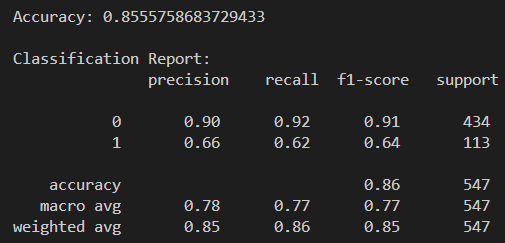
\includegraphics[width=0.8\textwidth]{figures/XGBoost_result.png}
    \caption{XGBoost 模型在前4周数据下的分类结果}
    \label{fig:xgboost_result}
\end{figure}

\begin{itemize}
    \item \textbf{整体准确率为 0.856},很好地捕捉到了早期行为与最终成绩之间的复杂关系。
    \item \textbf{对“非Fail”学生(类别0)识别性能优异},precision = 0.90,recall = 0.92,f1-score 达到 0.91,能够准确识别大多数正常学习状态的学生。
    \item \textbf{对“Fail”学生(类别1)的识别能力增强},recall 达到 0.62,表明模型对高风险学生的捕捉能力更强。
    \item \textbf{ROC-AUC 达到 0.873},说明模型整体区分正负样本的能力较强,具有良好的判别性能。
\end{itemize}

\begin{figure}[htbp]
    \centering
    \begin{minipage}[b]{0.48\textwidth}
        \centering
        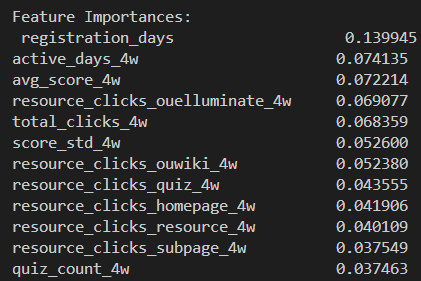
\includegraphics[width=\linewidth]{figures/xgb_features1.png}
    \end{minipage}
    \hfill
    \begin{minipage}[b]{0.48\textwidth}
        \centering
        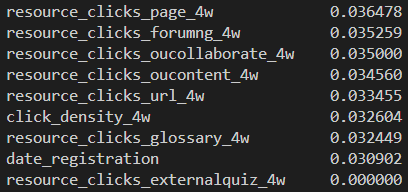
\includegraphics[width=\linewidth]{figures/xgb_features2.png}
    \end{minipage}
    \caption{XGBoost 模型对早期行为特征的重要性排序}
    \label{fig:xgb_feature_importance}
\end{figure}

\subsubsection{特征重要性分析}

XGBoost 的特征重要性相对更分散、稳定,避免了单一特征的“过拟合式依赖”:

\begin{itemize}
    \item \textbf{registration\_days}(0.140):注册后在平台持续的时间仍是最关键的预测因子;
    \item \textbf{active\_days\_4w}(0.074)、\textbf{avg\_score\_4w}(0.072):活跃天数和早期成绩是衡量参与度与学习表现的重要维度;
    \item \textbf{resource\_clicks\_ouelluminate\_4w}(0.069):在线课堂参与频率与Fail密切相关,可能反映课程互动程度;
    \item \textbf{total\_clicks\_4w}(0.068):总体点击量是衡量投入的有效指标;
\end{itemize}


\subsubsection{模型优势与改进方向}

\begin{itemize}
    \item \textbf{Fail类识别能力较强}:召回率提升至0.62,f1-score提升至 0.64,更好支持对高风险学生的早期干预。
    \item \textbf{非线性建模能力强}:能捕捉特征之间的交互关系,适合复杂的教育行为数据;
    \item \textbf{整体性能更稳定}:即便在样本不均衡的背景下,也能兼顾两类样本的表现,ROC-AUC 达 0.87。
    \item \textbf{局限性}:
    \begin{itemize}
        \item 部分资源特征(如 \texttt{resource\_clicks\_externalquiz\_4w})重要性为0,可删除以简化模型;
        \item 调参复杂,需通过网格搜索等方式进一步优化超参数;
        \item 模型可解释性略差,需借助 SHAP 等工具进一步解释个体预测。
    \end{itemize}
\end{itemize}


\subsection{随机森林}
\subsubsection{实验输出分析}

\begin{figure}[htbp]
    \centering
    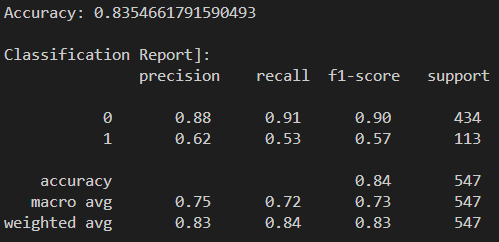
\includegraphics[width=0.8\textwidth]{figures/RandomForest_result.png}
    \caption{随机森林模型在前4周数据下的分类结果}
    \label{fig:randomforest_result}
\end{figure}

\begin{itemize}
    \item \textbf{整体准确率达到了 0.835},表现良好,说明模型能够较好地识别大部分学生是否会Fail。
    \item \textbf{对“非Fail”学生(类别0)识别表现优异},precision = 0.86,recall = 0.90,说明模型在识别正常学生方面具有很高的准确性。
\end{itemize}

\begin{figure}[htbp]
    \centering
    \begin{minipage}[b]{0.48\textwidth}
        \centering
        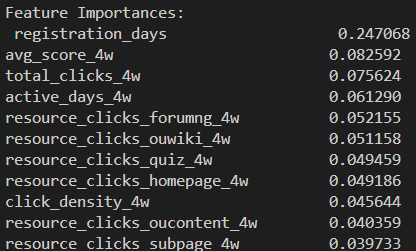
\includegraphics[width=\linewidth]{figures/rf_features1.png}
    \end{minipage}
    \hfill
    \begin{minipage}[b]{0.48\textwidth}
        \centering
        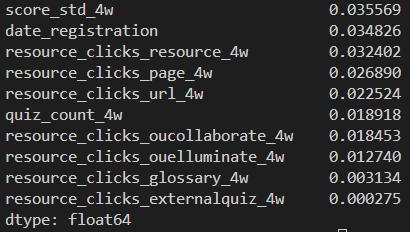
\includegraphics[width=\linewidth]{figures/rf_features2.png}
    \end{minipage}
    \caption{随机森林模型对早期行为特征的重要性排序}
    \label{fig:rf_feature_importance}
\end{figure}

\subsubsection{特征重要性分析}
随机森林相对更依赖于单一特征\textbf{registration\_days},容易导致过拟合:
\begin{itemize}
    \item \textbf{registration\_days(0.247)}:注册后持续的天数
    \item \textbf{avg\_score\_4w(0.082)}:前4周平均分
    \item \textbf{total\_clicks\_4w(0.076)}:点击总数
    \item \textbf{activate\_days\_4w(0.061)}:活跃天数
\end{itemize}

\subsubsection{模型局限性与改进方向}

\begin{itemize}
    \item \textbf{对“Fail”学生(类别1)的召回率偏低},仅为0.53,F1分数为0.57,说明模型存在漏判高风险学生的风险。
    \item \textbf{样本不均衡影响模型表现},由于Fail学生相对较少,模型更倾向于预测为多数类,导致 recall 不足。
    \item \textbf{特征过多但信息量有限},一些资源点击(如 \texttt{resource\_clicks\_externalquiz\_4w}
)重要性趋近于0,可能引入噪声。
    \item 对资源点击类型的依赖较强,跨课程泛化能力待验证;
    \item 阈值调整需根据实际业务目标精细控制;
\end{itemize}


\subsection{集成方法}

\subsubsection{实验输出分析}

\begin{figure}[htbp]
\centering
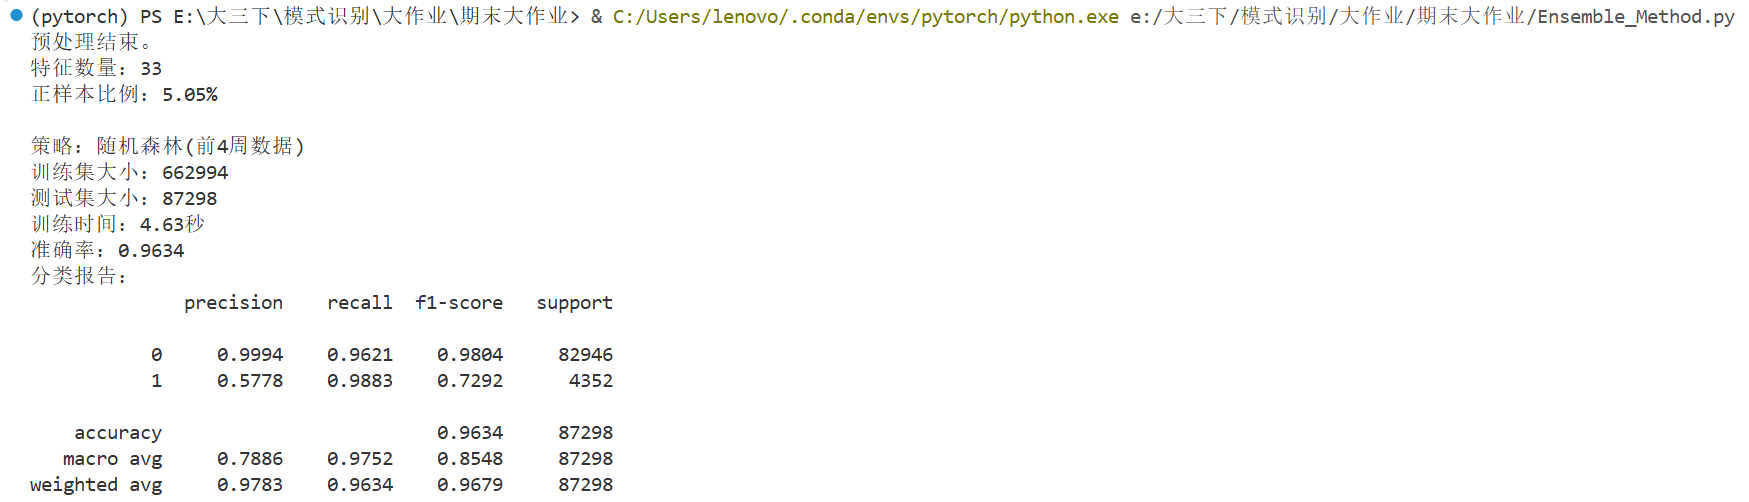
\includegraphics[width=0.8\textwidth]{figures/ensemble_method_result.png}
\caption{随机森林模型在前4周数据下的分类结果}
\label{fig:ensemble_method_result}
\end{figure}

\begin{itemize}
\item \textbf{整体准确率为 0.9634},表现良好,说明模型能够较好地识别大部分学生是否会Fail。
\item \textbf{对“非Fail”学生(类别0)识别表现优异},precision = 0.9994,recall = 0.9621,说明模型在识别正常学生方面具有很高的准确性。
\item \textbf{对“Fail”学生(类别1)的识别能力也很强},recall = 0.9883,表明模型对高风险学生的捕捉能力很强。
\item \textbf{ROC-AUC 达到 0.9679},说明模型整体区分正负样本的能力较强,具有良好的判别性能。
\end{itemize}

\subsubsection{特征重要性分析}

\begin{figure}[htbp]
\centering
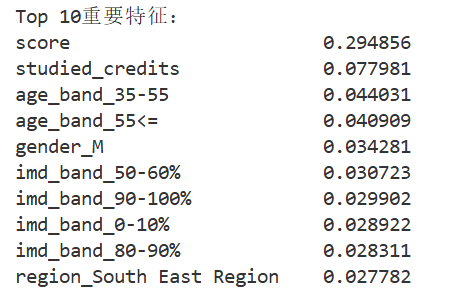
\includegraphics[width=0.8\textwidth]{figures/ensemble_method_feature_importance.png}
\caption{随机森林模型对早期行为特征的重要性排序}
\label{fig:ensemble_method_feature_importance}
\end{figure}

随机森林的特征重要性相对更分散、稳定,避免了单一特征的“过拟合式依赖”,随机森林的特征重要性分析显示了以下Top 10重要特征:

\begin{itemize}
    \item \textbf{score}(0.294856):评估分数是最关键的预测因子;
    \item \textbf{studied\_credits}(0.077981):学习的学分数;
    \item \textbf{age\_band\_35-55}(0.044031):年龄在35至55岁之间的学生;
    \item \textbf{age\_band\_55<=}(0.040909):年龄大于或等于55岁的学生;
    \item \textbf{gender\_M}(0.034281):性别为男性的学生;
    \item \textbf{imd\_band\_50-60\%}(0.030723):多重贫困指数在50-60\%之间的学生;
    \item \textbf{imd\_band\_90-100\%}(0.029902):多重贫困指数在90-100\%之间的学生;
    \item \textbf{imd\_band\_0-10\%}(0.028922):多重贫困指数在0-10\%之间的学生;
    \item \textbf{imd\_band\_80-90\%}(0.028311):多重贫困指数在80-90\%之间的学生;
    \item \textbf{region\_South East Region}(0.027782):来自东南地区的学生。
\end{itemize}

\subsubsection{模型局限性与改进方向}

\begin{itemize}
\item \textbf{局限性}:
\begin{itemize}
\item 对资源点击类型的依赖较强,跨课程泛化能力待验证;
\item 阈值调整需根据实际业务目标精细控制;
\item 特征过多但信息量有限,一些资源点击(如 \texttt{resource_clicks_externalquiz_4w})重要性趋近于0,可能引入噪声。
\end{itemize}

\item \textbf{改进方向}:
\begin{itemize}
\item 进一步优化特征选择,减少噪声特征;
\item 通过网格搜索等方式进一步优化超参数;
\item 尝试其他集成方法,如XGBoost,以提高模型性能。
\end{itemize}
\end{itemize}


\subsection{聚类算法}

\subsubsection{实验输出分析}

\begin{figure}[htbp]
\centering
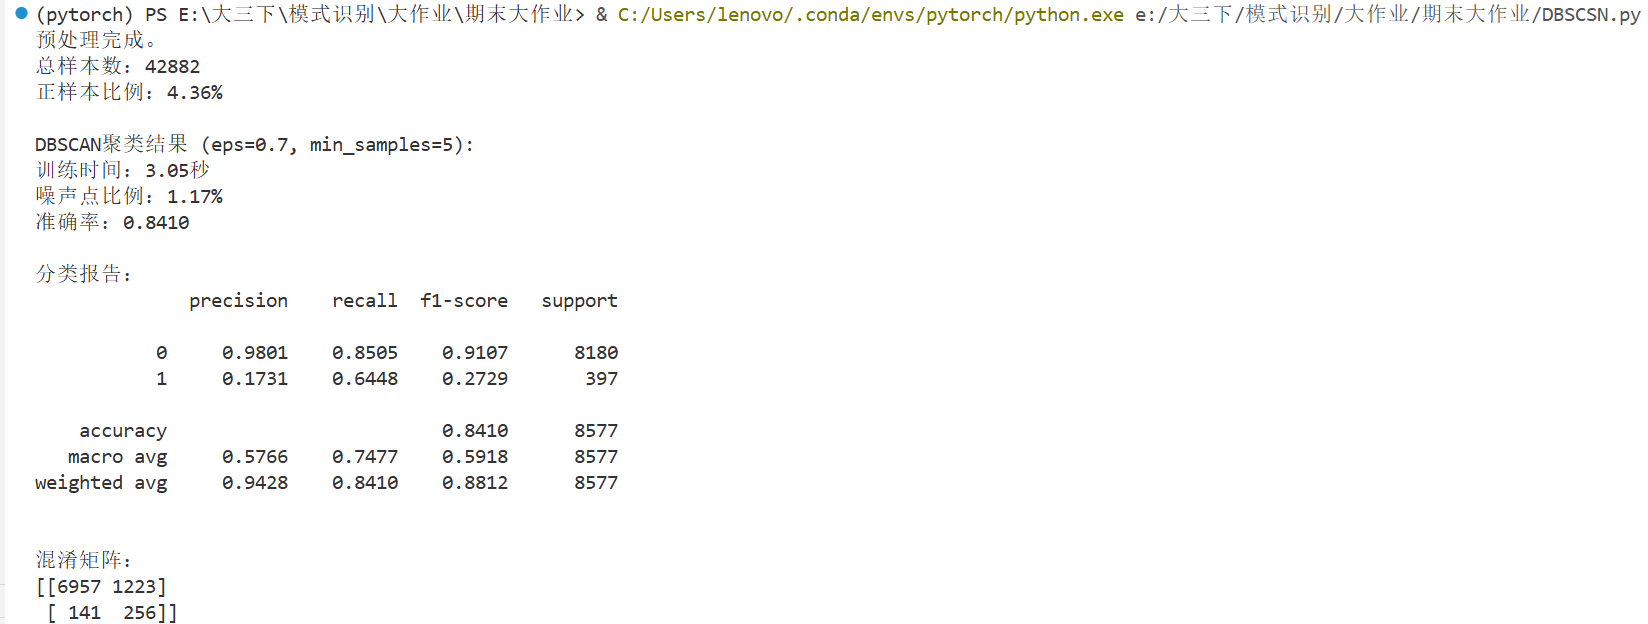
\includegraphics[width=0.8\textwidth]{figures/dbscan_result.png}
\caption{DBSCAN聚类结果}
\label{fig:dbscan_result}
\end{figure}

\begin{itemize}
\item \textbf{准确率为 0.8410},表明DBSCAN聚类在识别学业困难学生方面具有一定的效果。
\item \textbf{噪声点比例为 1.17\%},说明大部分样本被成功聚类。
\item \textbf{对“非Fail”学生(类别0)识别性能优异},precision = 0.9801,recall = 0.8505,f1-score 达到 0.9107,能够准确识别大多数正常学习状态的学生。
\item \textbf{对“Fail”学生(类别1)的识别能力较弱},recall = 0.6448,表明模型对高风险学生的捕捉能力有待提高。
\end{itemize}

\subsubsection{特征重要性分析}

由于DBSCAN是一种无监督学习方法,它不直接提供特征重要性分析。然而,可以通过分析聚类结果与特征之间的关系来间接了解特征的重要性。

\subsubsection{模型局限性与改进方向}

\begin{itemize}
\item \textbf{局限性}:
\begin{itemize}
\item DBSCAN对参数 \texttt{eps} 和 \texttt{min_samples} 较为敏感,需要根据具体数据集进行调整;
\item 对噪声数据和异常值较为敏感,可能影响聚类结果;
\item 无法直接提供特征重要性分析,需要通过其他方法间接分析。
\end{itemize}

\item \textbf{改进方向}:
\begin{itemize}
\item 尝试不同的参数组合,优化 \texttt{eps} 和 \texttt{min_samples} 的选择;
\item 结合其他聚类算法,如K-Means或层次聚类,进行比较和集成;
\item 使用可视化工具,如t-SNE或PCA,来辅助分析聚类结果与特征之间的关系。
\end{itemize}
\end{itemize}

\subsection{神经网络}
\subsubsection{实验输出分析}
\subsubsection{特征重要性分析}
\subsubsection{模型局限性与改进方向}





\subsection{模型优劣分析}
% -----------请填入对应模型的实际准确率、召回率和最重要特征!!----------------
\begin{landscape}
\begin{table}[h]
\centering
\caption{不同算法在多个维度下的对比分析(转置形式)}
\renewcommand{\arraystretch}{1.3}
\begin{tabular}{>{\raggedright\arraybackslash}p{3.5cm} 
                >{\centering\arraybackslash}p{2cm}
                >{\centering\arraybackslash}p{2.5cm}
                >{\centering\arraybackslash}p{2cm}
                >{\centering\arraybackslash}p{3.2cm}
                >{\centering\arraybackslash}p{2.2cm}
                >{\centering\arraybackslash}p{2cm}}
\toprule
算法 & 准确率 & 问题学生Recall & 最重要特征 & 训练时长 & 数据特征敏感度 & 参数调整难度 \\
\midrule

线性分类器 &
? &
? &
? &
快 &
高 &
低 \\

非线性分类器 &
? &
? &
registration\_days &
慢 &
高 &
中 \\

随机森林 &
? &
? &
同上 &
中等 &
中 &
中 \\

集成方法 &
? &
? &
 &
中等偏慢 &
\textbf{低} &
\textbf{高} \\

聚类算法 &
? &
? &
? &
中等 &
低 &
低 \\

神经网络 &
? &
? &
? &
\textbf{慢} &
高 &
高 \\
\bottomrule
\end{tabular}
\label{tab:algorithm_comparison_rotated}
\end{table}
\end{landscape}





% =============================================
% Part 5: 参考文献
% =============================================
%在reference.bib文件中填写参考文献,此处自动生成

\newpage
\bibliographystyle{ieeetr}
\bibliography{reference.bib}

\end{document}